\documentclass[aoas]{imsart}

%% Packages
\RequirePackage{amsthm,amsmath,amsfonts,amssymb}
\RequirePackage{natbib}
\RequirePackage[colorlinks,citecolor=blue,urlcolor=blue]{hyperref}
\RequirePackage{graphicx}
\RequirePackage{bm}

\DeclareMathOperator*{\argmax}{arg\,max}
\DeclareMathOperator*{\argmin}{arg\,min}

\startlocaldefs
%%%%%%%%%%%%%%%%%%%%%%%%%%%%%%%%%%%%%%%%%%%%%%
%%                                          %%
%% Uncomment next line to change            %%
%% the type of equation numbering           %%
%%                                          %%
%%%%%%%%%%%%%%%%%%%%%%%%%%%%%%%%%%%%%%%%%%%%%%
%\numberwithin{equation}{section}
%%%%%%%%%%%%%%%%%%%%%%%%%%%%%%%%%%%%%%%%%%%%%%
%%                                          %%
%% For Axiom, Claim, Corollary, Hypothesis, %%
%% Lemma, Theorem, Proposition              %%
%% use \theoremstyle{plain}                 %%
%%                                          %%
%%%%%%%%%%%%%%%%%%%%%%%%%%%%%%%%%%%%%%%%%%%%%%
\theoremstyle{plain}
\newtheorem{axiom}{Axiom}
\newtheorem{claim}[axiom]{Claim}
\newtheorem{theorem}{Theorem}[section]
\newtheorem{lemma}[theorem]{Lemma}
%%%%%%%%%%%%%%%%%%%%%%%%%%%%%%%%%%%%%%%%%%%%%%
%%                                          %%
%% For Assumption, Definition, Example,     %%
%% Notation, Property, Remark, Fact         %%
%% use \theoremstyle{remark}                %%
%%                                          %%
%%%%%%%%%%%%%%%%%%%%%%%%%%%%%%%%%%%%%%%%%%%%%%
\theoremstyle{remark}
\newtheorem{definition}[theorem]{Definition}
\newtheorem*{example}{Example}
\newtheorem*{fact}{Fact}
%%%%%%%%%%%%%%%%%%%%%%%%%%%%%%%%%%%%%%%%%%%%%%
%% Please put your definitions here:        %%
%%%%%%%%%%%%%%%%%%%%%%%%%%%%%%%%%%%%%%%%%%%%%%

\endlocaldefs

\begin{document}

\begin{frontmatter}
\title{Dynamic modeling of spike count data with Conway-Maxwell Poisson variability}
\runtitle{Dynamic CMP model for neural activities}

\begin{aug}
%%%%%%%%%%%%%%%%%%%%%%%%%%%%%%%%%%%%%%%%%%%%%%%
%% Only one address is permitted per author. %%
%% Only division, organization and e-mail is %%
%% included in the address.                  %%
%% Additional information can be included in %%
%% the Acknowledgments section if necessary. %%
%%%%%%%%%%%%%%%%%%%%%%%%%%%%%%%%%%%%%%%%%%%%%%%
%\author[A]{\fnms{Ganchao} \snm{Wei}\ead[label=e1, mark]{ganchao.wei@uconn.edu}}
\author{\fnms{Ganchao} \snm{Wei}\ead[label=e1, mark]{ganchao.wei@uconn.edu}}
\and
%\author{\fnms{Ian H.} \snm{Stevenson}\ead[label=e2]{ian.stevenson@uconn.edu}}
\author{\fnms{Ian H.} \snm{Stevenson}\ead[label=e2]{ian.stevenson@uconn.edu}}
%%%%%%%%%%%%%%%%%%%%%%%%%%%%%%%%%%%%%%%%%%%%%%
%% Addresses                                %%
%%%%%%%%%%%%%%%%%%%%%%%%%%%%%%%%%%%%%%%%%%%%%%
\address{University of Connecticut,
\printead{e1}}

%\address[B]{Department of Psychological Sciences,
%University of Connecticut}
%
%\address[C]{Department of Biomedical Engineering, University of Connecticut}
%
%\address[D]{Connecticut Institute for Brain and Cognitive Science,
%	University of Connecticut,
%	\printead{e2}}
\end{aug}

\begin{abstract}
The abstract should summarize the contents of the paper.
It should be clear, descriptive, self-explanatory and not longer
than 200 words. It should also be suitable for publication in
abstracting services. Formulas should be used as sparingly as
possible within the abstract. The abstract should not make
reference to results, bibliography or formulas in the body
of the paper---it should be self-contained.

This is a sample input file.  Comparing it with the output it
generates can show you how to produce a simple document of
your own.
\end{abstract}

\begin{keyword}
\kwd{First keyword}
\kwd{second keyword}
\end{keyword}

\end{frontmatter}
%%%%%%%%%%%%%%%%%%%%%%%%%%%%%%%%%%%%%%%%%%%%%%
%% Please use \tableofcontents for articles %%
%% with 50 pages and more                   %%
%%%%%%%%%%%%%%%%%%%%%%%%%%%%%%%%%%%%%%%%%%%%%%
%\tableofcontents

\section{Introduction}



\section{Methods}
Here we consider a dynamic GLM with Conway-Maxwell Poisson (CMP) observations to describe time-varying spike counts. We first introduce the model. Although the CMP distribution allows us to flexibly model non-Poisson variability, one major challenge with using this model is that there are not closed-form solutions for the CMP likelihood. Here, we infer fit the model using a global Gaussian approximation, and we discuss several additional technical challenges that arise when using the CMP distribution with a dynamic GLM.

\subsection{Dynamic Conway-Maxwell Poisson Model}
A count observation $y$, such as the spike count for a neuron, is assumed to follow the CMP distribution, with parameters $\lambda$ and $\nu$. The probability mass function (pmf) of CMP distribution is:
\begin{equation}
	P(Y=y|\lambda, \nu) = \frac{\lambda^y}{(y!)^\nu}\cdot\frac{1}{Z(\lambda, \nu)}
\end{equation}
, where $Z(\lambda, \nu)=\sum_{k=0}^{\infty}\frac{\lambda^k}{(k!)^\nu}$ is the normalizing constant. The parameter $\nu \geq 0$ controls different dispersion patterns, i.e. equi- $(\nu=1)$, over- $(0\leq\nu<1)$ or under-dispersion $(\nu > 1)$. Three common distributions occur as special cases: 1) the Poisson $(\nu=1)$, 2) the geometric $(\nu=0, \lambda<1)$, and 3) the Bernoulli $(\nu \rightarrow \infty)$.

For multiple observations up to T steps, such as simultaneous spike counts from n neurons, denote the counts at time bin $t$ as $\bm{y}_t = (y_{1t},\ldots,y_{nt})'$, for $t=1,\ldots, T$. The corresponding CMP parameters at $t$ are $\bm{\lambda}_t = (\lambda_{1t},\ldots,\lambda_{nt})'$ and $\bm{\nu}_t = (\nu_{1t},\ldots,\nu_{nt})'$. Previous work has examined the CMP-GLM (\cite{Chatla2018,Sellers2010}), and here we focus on the dynamic version of this GLM. The CMP parameters at $t$ are modeled by two log-linear models, $\log\bm{\lambda}_t = \bm{X}_t\bm{\beta}_t$ and $\log\bm{\nu}_t = \bm{G}_t\bm{\gamma}_t$, with $\bm{\beta}_t \in \mathbb{R}^p$ and $\bm{\gamma}_t \in \mathbb{R}^q$, and $\bm{X}_t$ and $\bm{G}_t$ denote known predictors. Under the CMP-GLM, the parameters are static. Here, we assume that they  progress linearly with a Gaussian noise.

The observations follow conditionally independent CMP distributions, given the state vector $\bm{\theta}_t = (\bm{\beta}'_t, \bm{\gamma}'_t)'$. 
\begin{align}
	\bm{y}_t &\sim CMP(\bm{\lambda}_t, \bm{\nu}_t)\\
	\log\bm{\lambda}_t &= \bm{X}_t\bm{\beta}_t, \quad \log\bm{\nu}_t = \bm{G}_t\bm{\gamma}_t \nonumber
\end{align}

While the state vector  $\bm{\theta}_t$ evolves linearly with Gaussian noise:
\begin{align}
	\bm{\theta}_1 &\sim N_{p+q}(\bm{\theta}_0, \bm{Q}_0)\\
	\bm{\theta}_t|\bm{\theta}_{t-1} &\sim N_{p+q}(\bm{F\theta}_{t-1}, \bm{Q}) \nonumber
\end{align}
Given the initial state mean $\bm{\theta}_0$, covariance $\bm{Q}_0$, linear dynamics $\bm{F}$ and process covariance $\bm{Q}$.

\subsubsection{Inference by Gaussian approximation}
To fit the model to data we need to estimate the time-varying state vector $\bm{\Theta} = (\bm{\theta}'_1,\ldots,\bm{\theta}'_T)\in\mathbb{R}^{(p+q)T}$. In this section, we first assume $\bm{F}$ and $\bm{Q}$ are known. Since the observations are CMP distributed, we cannot estimate $\bm{\Theta}$ in closed form. Instead, here we approximate it by a multivariate Gaussian distribution, $P(\bm{\Theta|Y}) \approx N_{(p+q)T}(\bm{\Theta|,\mu,\Sigma})$, with $\bm{Y} = (\bm{y}'_1,\ldots, \bm{y}'_T)'$. The parameters of this Gaussian are found by a global Laplace approximation, i.e. $\bm{\mu} = \argmax_{\bm{\Theta}}P(\bm{\Theta|Y})$ and $\bm{\Sigma} = -(\nabla\nabla_{\bm{\Theta}}\log P(\bm{\Theta|Y})|_{\bm{\Theta - \mu}})^{-1}$. The log-posterior is given by:
\begin{align}
	\log P(\bm{\Theta|Y}) &= \sum_{t=1}^{T}l_t - \frac{1}{2}(\bm{\theta}_1 - \bm{\theta}_0)'\bm{Q}_0^{-1}(\bm{\theta}_1 - \bm{\theta}_0) - \frac{1}{2}\sum_{t=2}^{T}(\bm{\theta}_t - \bm{F\theta}_{t-1})'\bm{Q}^{-1}(\bm{\theta}_t - \bm{F\theta}_{t-1})\\
	l_t &= l(\bm{\theta}_t) = \log P(\bm{y}_t|\bm{\theta}_t) = \sum_{i=1}^{n}y_{it}\log \lambda_{it} - \nu_{it}y_{it}! - \log Z(\lambda_{it}, \nu_{it}) \nonumber
\end{align}
, where $l(\cdot)$is the log-likelihood. The log-posterior is concave (\cite{Gupta2014}), and the Markovian structure of the state vector dynamics makes it possible to optimize by Newton-Raphson (NR) in $\mathcal{O}(T)$ time (\cite{Paninski2010}).After the Newton update, we can further quantify the uncertainty for the CMP parameters and the underlying rates, as in Appendix \ref{appA}.

There are several technical challenges involved with performing the Newton update with CMP observations. Firstly, in order to find the gradient and Hessian we need to calculate moments of $Y_{it}$ and $\log Y_{it}!$, which have no closed forms (\cite{Shmueli2005}). We can calculate these moments by truncated summation. However, when $\lambda \geq 2$ and $\nu \leq 1$,  truncated summation is computationally costly since we need many steps for accurate approximation. In this case, we approximate the moments using previous (\cite{Chatla2018,Gaunt2019}) asymptotic results as in Appendix \ref{appB}. A second challenge is that the Hessian is not robust to outliers. Outliers often result in the Hessian being close to singular or even positive-definite. See details in Appendix \ref{appC}. To ensure robustness, we use Fisher scoring where the observed information is replaced by the expected information. Finally, a third challenge is that the Newton updates take a long time to converge if the initial state estimate is far from the maximum of the posterior, especially when $T$ is large. To resolve this issue, we use a smoothing estimate with local Gaussian approximation as a “warm start”. Forward filtering for a dynamic Poisson model has been previously described in \cite{Eden2004}, and here we implement CMP filtering following the same rationale. Let $\bm{\theta}_{t|t-1} = E(\bm{\theta}_t|\bm{y}_1,\ldots,\bm{y}_{t-1})$ and $\bm{\Sigma}_{t|t-1} = Var(\bm{\theta}_t|\bm{y}_1,\ldots,\bm{y}_{t-1})$ be the mean and variance for the one-step prediction density and $\bm{\theta}_{t|t} = E(\bm{\theta}_t|\bm{y}_1,\ldots,\bm{y}_{t})$ and $\bm{\Sigma}_{t|t} = Var(\bm{\theta}_t|\bm{y}_1,\ldots,\bm{y}_t)$ be mean and variance for the posterior density, then the filtering update for step $t$ is given by
\begin{align}
	\bm{\theta}_{t|t-1} &= \bm{F\theta}_{t-1|t-1}\\
	\bm{\Sigma}_{t|t-1} &= \bm{F\Sigma}_{t-1|t-1}\bm{F}' + \bm{Q} \nonumber\\
	\bm{\theta}_{t|t} &= \bm{\theta}_{t|t-1} + (\bm{\Sigma}_{t|t})\left[\frac{\partial l_t}{\partial \bm{\theta}_t}\right]_{\bm{\theta}_{t|t-1}} \nonumber\\
	(\bm{\Sigma}_{t|t})^{-1} &= (\bm{\Sigma}_{t|t-1})^{-1} - \left[\frac{\partial^2l_t}{\partial\bm{\theta}_t\partial\bm{\theta}'_t}\right]_{\bm{\theta}_{t|t-1}} \nonumber
\end{align}
Here, to again ensure robustness, we use Fisher scoring when updating the state covariance. We then find smoothed estimates using a backward pass (\cite{RAUCH1965}). Although doing smoothing is fast, the estimates can be inaccurate, especially when there are large changes in the state vector. In the forward filtering stage, the Gaussian approximation at each step $t$ is conducted locally at the recursive prior $\bm{\theta}_{t|t-1}$. This will be statistically inefficient when the recursive prior is too far away from the posterior mode, or when there is a large change in the state vector. Moreover, Fisher scoring reduces the efficiency of the smoother even further. The smoother provides reasonable initial estimates, but estimation accuracy is substantially improved by using Newton’s method to find the global Laplace approximation for the posterior.

\subsubsection{Estimating process noise}
For the applications to neural data examined here, we assume that $\bm{F}=\bm{I}$. However, we still need to estimate the process noise $\bm{Q}$. When $n$ is small, especially when $n=1$, different $\bm{Q}$ values will have a substantial influence on estimation. One possible way to estimate. One possible way to estimate $\bm{Q}$ is to use an Expectation Maximization (EM) algorithm as in \cite{Macke2011}. However, using the Laplace approximation for $\bm{\Theta}$ during E-step breaks the usual guarantee of non-decreasing likelihoods in EM, and, hence, may lead to divergence. To avoid that, we could sample the posterior directly by MCMC. However, the lack of closed-form moments for the CMP distribution makes sampling computationally intensive. Here, to estimate $\bm{Q}$ robustly and quickly, we instead assume $\bm{Q}$ is diagonal and estimate it by maximizing the prediction likelihood in the filtering stage, as in \cite{Wei2021}. 


\subsubsection{Neural Data}

\textcolor{red}{I prefer to move this section to application part (reason: this is the data we use, but the not the method we propose. If we collect the data by ourself, surely we should write it here. But we are just using it $\ldots$)}

\section{Simulation}
TBD

\subsection{Figure 1}
\begin{figure}[h!]
	\centering
	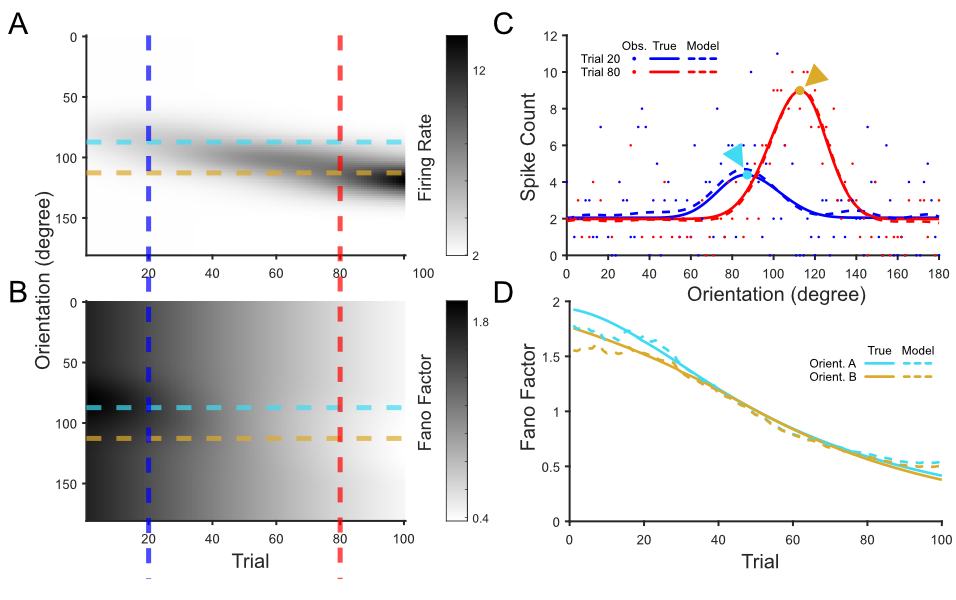
\includegraphics[width=1\textwidth]{figure1.png}
	\caption{A simulated neuron with a shifting firing pattern.}
	\label{fig1}
\end{figure}

\subsection{Figure 2}
\begin{figure}[h!]
	\centering
	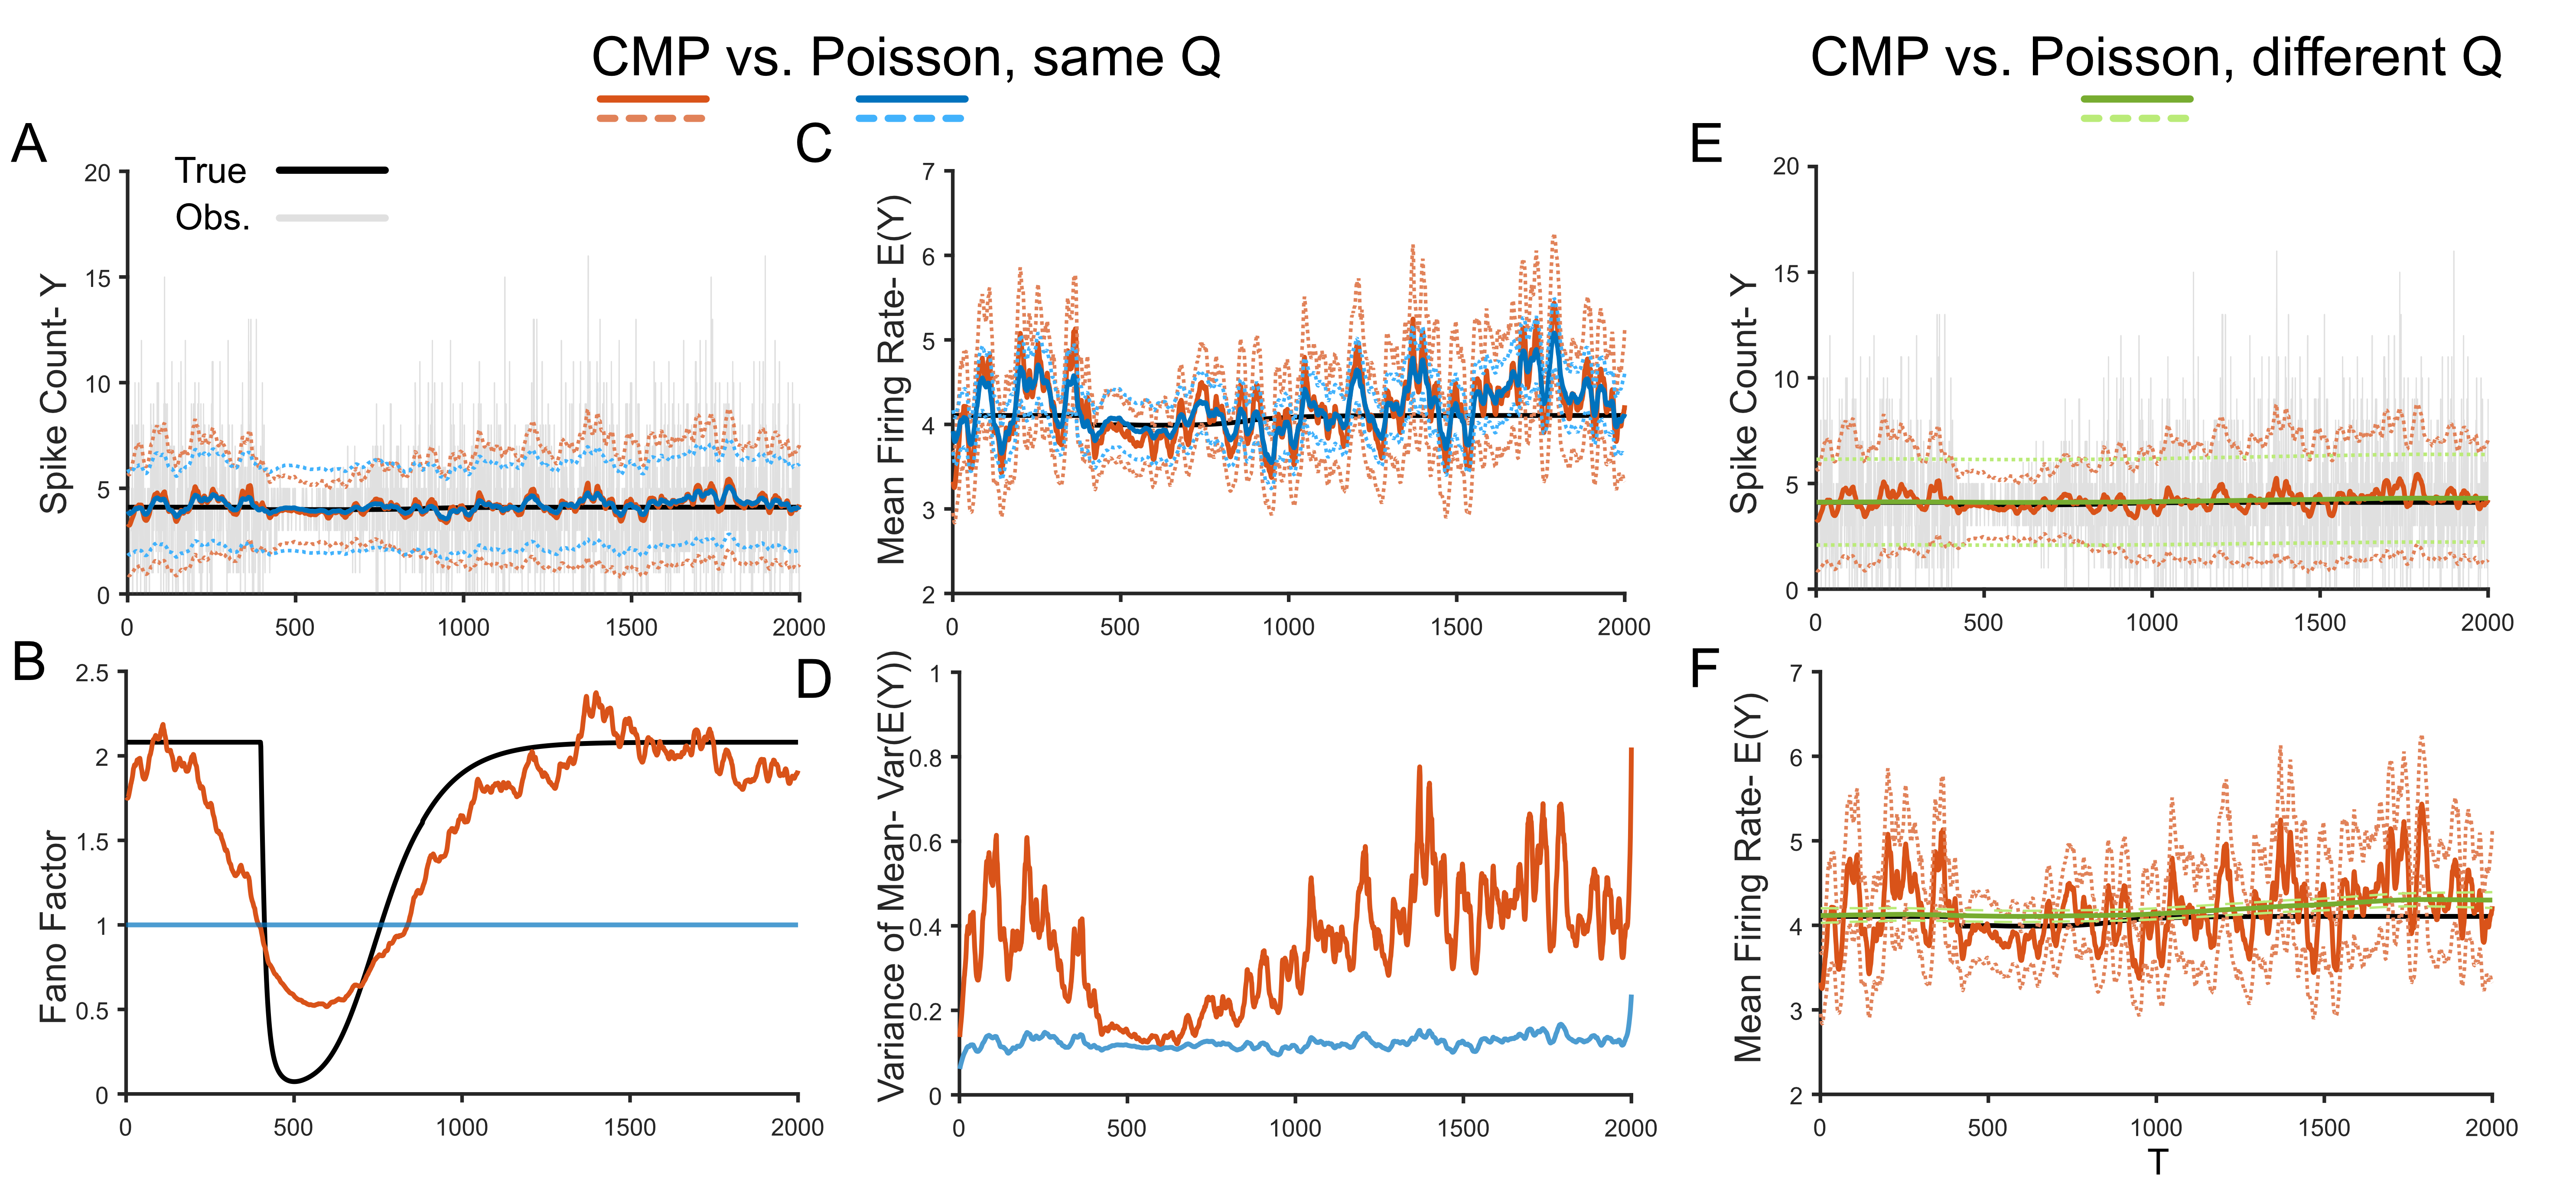
\includegraphics[width=1\textwidth]{figure2_new.png}
	\caption{Constant firing rate with non-stationary variability.}
	\label{fig2}
\end{figure}

\section{Application}
TBD

\subsection{V1 data}
TBD

\subsection{HC data}
TBD


%%%%%%%%%%%%%%%%%%%%%%%%%%%%%%%%%%%%%%%%%%%%%%

%% Example with multiple Appendixes:        %%
%%%%%%%%%%%%%%%%%%%%%%%%%%%%%%%%%%%%%%%%%%%%%%
\begin{appendix}
\section{Quantifying Uncertainties}\label{appA}

After convergence, we have an approximation of the log-posterior $P(\bm{\theta}_t|\bm{Y}) \approx N(\bm{\theta}_t|\bm{\mu}_t, \bm{\Sigma}_t)$, and we can use this approximation to quantify the uncertainty about the CMP parameters, as well as about the mean rate at each time.

The CMP parameters are log-normal distributed. Let $\bm{Z}_{it} = \begin{pmatrix}
	\bm{x}'_{it} & \bm{0} \\
	\bm{0} & \bm{g}'_{it} 
\end{pmatrix}$, then $(\lambda_{it},\nu_{it})'=\exp(\bm{Z}_{it}\bm{\theta}_t) \sim \text{Lognormal}_2(\bm{Z}_{it}\bm{\mu}_t, \bm{Z}_{it}\bm{\Sigma}_t\bm{Z}'_{it})$. Denote the variance of CMP parameters as $\bm{V}_{it}$. \textcolor{red}{The variance can be easily found in Wiki. If I write it out, I need to define some useless notations. See Word Documents}.

The conditional mean firing rate is $\delta_{it} = E(Y_{it})$, whose variance can be calculated by the Delta method:
\begin{align}
	\widehat{Var}(\delta_{it}) &=  \begin{pmatrix}
		\frac{\partial\delta_{it}}{\partial\lambda_{it}} & \frac{\partial\delta_{it}}{\partial\nu_{it}} 
	\end{pmatrix}\bm{V}_{it}\begin{pmatrix}
	\frac{\partial\delta_{it}}{\partial\lambda_{it}} \\ \frac{\partial\delta_{it}}{\partial\nu_{it}}
\end{pmatrix}\\
\frac{\partial\delta_{it}}{\partial\lambda_{it}} &= \frac{\partial^2\log Z_{it}}{\partial\log\lambda_{it}\partial\lambda_{it}} = \frac{Var(Y_{it})}{\lambda_{it}}\\
\frac{\partial\delta_{it}}{\partial\nu_{it}} &= \frac{\partial^2\log Z_{it}}{\partial\log\lambda_{it}\partial\nu_{it}} = -Cov(Y_{it}, \log Y_{it}!)
\end{align}
We can calculate the moments as in Appendix \ref{appB}, or we can use simpler approximations $E(Y) = \lambda^{1/\nu} - \frac{\nu-1}{2\nu}$ when $\nu\leq 1$ or $\lambda > 10^\nu$. Then $\frac{\partial\delta_{it}}{\partial\lambda_{it}}\approx\frac{1}{\nu_{it}}\lambda_{it}^{1/\nu_{it} - 1}$ and $\frac{\delta_{it}}{\nu_{it}} \approx -\frac{\lambda_{it}^{1/\nu_{it}}\log \lambda_{it}}{\nu_{it}^2} - \frac{1}{2\nu_{it}^2}$.

\section{Moments approximation for Conway-Maxwell Poisson distribution}\label{appB}
To estimate the state-vector for the dynamic CMP model, we need to find first and second moments for $Y$ and $\log Y!$. For $Y\sim CMP(\lambda, \nu)$,
\begin{align}
	Z(\lambda, \nu) &= \sum_{k=0}^{\infty}\frac{\lambda^k}{(k!)^\nu}\\
	E(Y) &= \frac{\partial\log Z}{\partial \log\lambda} = \frac{1}{Z}\sum_{k=0}^{\infty}\frac{k\lambda^k}{(k!)^\nu} \nonumber\\
	Var(Y) &= \frac{\partial^2\log Z}{\partial(\log \lambda)^2} = \frac{1}{Z}\sum_{k=0}^{\infty}\frac{k^2\lambda^k}{(k!)^\nu} - E^2(Y) \nonumber\\
	E(\log Y!) &= -\frac{\partial\log Z}{\partial\nu} = \frac{1}{Z}\sum_{k=0}^{\infty}\frac{(\log k!)\lambda^k}{(k!)^\nu} \nonumber\\
	Var(\log Y!) &= \frac{\partial^2\log Z}{\partial \nu^2} = \frac{1}{Z}\sum_{k=0}^{\infty}\frac{(\log k!)^2\lambda^k}{(k!)^\nu} - E^2(\log Y!) \nonumber\\
	Cov(Y, \log Y!) &= -\frac{\partial^2\log Z}{\partial \log\lambda\partial\nu} = \frac{1}{Z}\sum_{k=0}^{\infty}\frac{(\log k!) k\lambda^k}{(k!)^\nu} - E(\log Y!)E(Y) \nonumber
\end{align}
Generally, these moments can be calculated by truncated summation.

However, when $\lambda \geq 2$ and $\nu \leq 1$, we need many steps for accurate approximation. In this case, we make use of a previous asymptotic results for efficient calculation. Let $\alpha = \lambda^{1/\nu}, c_1 = \frac{\nu^2-1}{24}$ and $c_2 = \frac{\nu^2 - 1}{48} + \frac{c_1^2}{2}$,

\begin{equation}
	Z(\lambda, \nu)=\frac{e^{\nu\alpha}}{\lambda^{\frac{\nu-1}{2\nu}}(2\pi)^\frac{\nu-1}{2}\sqrt{\nu}}(1+c_1(\nu\alpha)^{-1} + c_2(\nu\alpha)^{-2} + \mathcal{O}(\lambda^{-3/\nu}))
\end{equation}
Then the moments are:
\begin{align}
	E(Y) &= \alpha - \frac{\nu-1}{2\nu} - \frac{\nu^2-1}{24\nu^2}\alpha^{-1}-\frac{\nu^2-1}{24\nu^3}\alpha^{-2} + \mathcal{O}(\alpha^{-3})\\
	Var(Y) &= \frac{\alpha}{\nu} + \frac{\nu^2-1}{24\nu^3}\alpha^{-1} + \frac{\nu^2-1}{12\nu^4}\aleph^{-2} + \mathcal{O}(\alpha^{-3}) \nonumber\\
	E(\log Y!) &= \alpha\left(\frac{\log\lambda}{\nu} - 1\right) + \frac{\log\lambda}{2\nu^2} + \frac{1}{2\nu} + \frac{\log 2\pi}{2} \nonumber \\
	&- \frac{\alpha^{-1}}{24}\left(1 + \frac{1}{\nu^2} + \frac{\log\lambda}{\nu} - \frac{\log\lambda}{\nu^3}\right) \nonumber\\
	&- \frac{\alpha^{-2}}{24}\left(\frac{1}{\nu^3} + \frac{\log\lambda}{\nu^2} - \frac{\log \lambda}{\nu^4}\right) + \mathcal{O}(\alpha^{-3}) \nonumber \\
	Var(\log Y!) &= \frac{\alpha(\log\lambda)^2}{\nu^3} + \frac{\log\lambda}{\nu^3} + \frac{1}{2\nu^2} \nonumber\\
	&+ \frac{\alpha^{-1}}{24\nu^5}[-2\nu^2 + 4\nu\log\lambda + (-1 + \nu^2)(\log\lambda)^2] \nonumber\\
	&+ \frac{\alpha^{-2}}{24\nu^6}[-3\nu^2 - 2\nu(-3 + \nu^2)\log\lambda + 2(-1 + \nu^2)(\log\lambda)^2] + \mathcal{O}(\alpha^{-3}) \nonumber \\
	Cov(Y, \log Y!) &= \frac{\alpha\log\lambda}{\nu^2} + \frac{1}{2\nu^2} + \frac{\alpha^{-1}}{24}\left(\frac{2}{\nu^3} + \frac{\log\lambda}{\nu^2} - \frac{\log\lambda}{\nu^4}\right) \nonumber\\
	&-\frac{1}{24\alpha^2}\left(\frac{1}{\nu^2} - \frac{3}{\nu^4} - \frac{2\log\lambda}{\nu^3} + \frac{2\log\lambda}{\nu^5}\right) + \mathcal{O}(\alpha^{-3}) \nonumber
\end{align}


\section{Gradient and Hessian of the log-posterior}\label{appC}
We estimate the state vector by maximizing the log-posterior with Newton-Raphson updates. Denote $f = P(\bm{\Theta|Y})$, the $(k+1)$-th update of NR algorithm is $\bm{\Theta}^{(k+1)} = \bm{\Theta}^{(k)} + [\nabla\nabla_{\bm{\Theta}^{(k)}}f]^{-1}\nabla_{\bm{\Theta}^{(k)}}f$. 
The gradient is:
\begin{align}
	\nabla_{\bm{\Theta}}f &= \left[\left(\frac{\partial f}{\partial \bm{\theta}_1}\right)',\ldots,\left(\frac{\partial f}{\partial \bm{\theta}_T}\right)'\right]'\\
	\frac{\partial f}{\partial\bm{\theta}_1} &= \frac{\partial l_1}{\partial\bm{\theta}_1} -  \bm{Q}_0^{-1}(\bm{\theta}_1 - \bm{\theta}_0)   +  \bm{F'Q}^{-1}(\bm{\theta}_2 - \bm{F\theta}_{1}) \nonumber\\
	\frac{\partial f}{\partial\bm{\theta}_t} &= \frac{\partial l_t}{\partial\bm{\theta}_t} -  \bm{Q}^{-1}(\bm{\theta}_t - \bm{F\theta}_{t-1})   +  \bm{F'Q}^{-1}(\bm{\theta}_{t+1} - \bm{F\theta}_{t}) \nonumber\\
	\frac{\partial f}{\partial\bm{\theta}_T} &= \frac{\partial l_T}{\partial\bm{\theta}_T} -  \bm{Q}^{-1}(\bm{\theta}_T - \bm{F\theta}_{T-1})    \nonumber\\
	\frac{\partial l_t}{\partial\bm{\theta}_t} &= \sum_{i = 1}^{n}\begin{pmatrix}
		{\left( y_{it} - E\left( Y_{it} \right) \right)\bm{x}}_{it} \\
		{\nu_{it}\left( E\left( \log{Y_{it}!} \right) - \log{y_{it}!} \right)\bm{g}}_{it} \\
	\end{pmatrix} \nonumber
\end{align}

The Hessian is:
\begin{align}
	\nabla\nabla_{\bm{\Theta}}f &=
	\begin{pmatrix}
		\frac{\partial^{2}f}{\partial\bm{\theta}_{1}\partial\bm{\theta}_{1}^{'}} & \bm{F}'\bm{Q}^{-1} &\bm{0} & \cdots & \bm{0} \\
		\bm{Q}^{- 1}\bm{F} & \frac{\partial^{2}f}{\partial\bm{\theta}_{2}\partial\bm{\theta}_{2}^{'}}&\bm{F}'\bm{Q}^{-1} & \cdots & \vdots \\
		\bm{0} & \bm{Q}^{-1}\bm{F}  & \frac{\partial^{2}f}{\partial\bm{\theta}_{3}\partial\bm{\theta}_{3}^{'}} & \cdots & \vdots\\
		\vdots & \vdots & \vdots & \ddots & \vdots \\
		\bm{0} & \cdots & \cdots & \cdots & \frac{\partial^{2}f}{\partial\bm{\theta}_{T}\partial\bm{\theta}_{T}^{'}}
	\end{pmatrix}\\
\frac{\partial^{2}f}{\partial\bm{\theta}_{1}\partial\bm{\theta}_{1}^{'}}  &= \frac{\partial^{2}l_1}{\partial\bm{\theta}_{1}\partial\bm{\theta}_{1}^{'}} - \bm{Q}_0^{-1} - \bm{F}'\bm{Q}^{-1}\bm{F} \nonumber\\
\frac{\partial^{2}f}{\partial\bm{\theta}_{t}\partial\bm{\theta}_{t}^{'}}  &= \frac{\partial^{2}l_t}{\partial\bm{\theta}_{t}\partial\bm{\theta}_{t}^{'}} - \bm{Q}^{-1} - \bm{F}'\bm{Q}^{-1}\bm{F} \nonumber\\
\frac{\partial^{2}f}{\partial\bm{\theta}_{T}\partial\bm{\theta}_{T}^{'}}  &= \frac{\partial^{2}l_T}{\partial\bm{\theta}_{T}\partial\bm{\theta}_{T}^{'}} - \bm{Q}^{-1} \nonumber
\end{align}
, where
\begin{align}
	\frac{\partial^{2}l_t}{\partial\bm{\theta}_{t}\partial\bm{\theta}_{t}^{'}} &= \sum_{i = 1}^{n}\begin{pmatrix}
		\bm{A}_{it} & \bm{B}_{it}\\
		\bm{B}'_{it} & \bm{C}_{it}
	\end{pmatrix}\\
\bm{A}_{it} &= Var(Y_{it})\bm{x}_{it}\bm{x}'_{it} \nonumber\\
\bm{B}_{it} &= -\nu_{it}Cov(Y_{it}, \log Y_{it}!)\bm{x}_{it}\bm{g}'_{it} \nonumber\\
\bm{C}_{it} &= \nu_{it}[\nu_{it}Var(\log Y_{it}) - E(\log Y_{it}!) + \log y_{it}!]\bm{g}_{it}\bm{g}'_{it} \nonumber
\end{align}

When $\log y_{it}! \ll E(\log Y_{it}!)$, the Hessian may be ill-conditioned or even positive-definite. To ensure the robustness, do Fisher scoring, i.e. replace the observed information $-\nabla\nabla_{\bm{\Theta}}f$ by the expected information $E(-\nabla\nabla_{\bm{\Theta}}f)$, so that $\bm{C}_{it} = \nu_{it}^2Var(\log Y_{it}!)\bm{g}_{it}\bm{g}'_{it}$
\end{appendix}

%%%%%%%%%%%%%%%%%%%%%%%%%%%%%%%%%%%%%%%%%%%%%%
%% Support information, if any,             %%
%% should be provided in the                %%
%% Acknowledgements section.                %%
%%%%%%%%%%%%%%%%%%%%%%%%%%%%%%%%%%%%%%%%%%%%%%
\begin{acks}[Acknowledgments]
The authors would like to thank the anonymous referees, an Associate
Editor and the Editor for their constructive comments that improved the
quality of this paper.
\end{acks}

%%%%%%%%%%%%%%%%%%%%%%%%%%%%%%%%%%%%%%%%%%%%%%
%% Funding information, if any,             %%
%% should be provided in the                %%
%% funding section.                         %%
%%%%%%%%%%%%%%%%%%%%%%%%%%%%%%%%%%%%%%%%%%%%%%
\begin{funding}
This material is based upon work supported by the National Science Foundation under Grant No. 1931249.
	
The first author was supported by NSF Grant DMS-??-??????.

The second author was supported in part by NIH Grant ???????????.
\end{funding}

%%%%%%%%%%%%%%%%%%%%%%%%%%%%%%%%%%%%%%%%%%%%%%
%% Supplementary Material, including data   %%
%% sets and code, should be provided in     %%
%% {supplement} environment with title      %%
%% and short description. It cannot be      %%
%% available exclusively as external link.  %%
%% All Supplementary Material must be       %%
%% available to the reader on Project       %%
%% Euclid with the published article.       %%
%%%%%%%%%%%%%%%%%%%%%%%%%%%%%%%%%%%%%%%%%%%%%%
\begin{supplement}
\stitle{Title of Supplement A}
\sdescription{Short description of Supplement A.}
\end{supplement}

%%%%%%%%%%%%%%%%%%%%%%%%%%%%%%%%%%%%%%%%%%%%%%%%%%%%%%%%%%%%%
%%                  The Bibliography                       %%
%%                                                         %%
%%  imsart-nameyear.bst  will be used to                   %%
%%  create a .BBL file for submission.                     %%
%%                                                         %%
%%  Note that the displayed Bibliography will not          %%
%%  necessarily be rendered by Latex exactly as specified  %%
%%  in the online Instructions for Authors.                %%
%%                                                         %%
%%  MR numbers will be added by VTeX.                      %%
%%                                                         %%
%%  Use \cite{...} to cite references in text.             %%
%%                                                         %%
%%%%%%%%%%%%%%%%%%%%%%%%%%%%%%%%%%%%%%%%%%%%%%%%%%%%%%%%%%%%%

%% if your bibliography is in bibtex format, uncomment commands:
\bibliographystyle{imsart-nameyear} % Style BST file
\bibliography{MyCollection}       % Bibliography file (usually '*.bib')

\end{document}
